\begin{task}

\TT{Na układ LTI o transmitancji podanej poniżej, podano sygnał $u(t)=A \cdot Sa\left(3 \cdot \omega_0 \cdot t\right)$. Wyznacz odpowied\'{z} układu $y(t)$ wiedząc, że $\Pi(t) \xrightarrow{\mathcal F} Sa\left(\frac{\omega}{2}\right)$.}{A signal $u(t)=A \cdot Sa\left(3 \cdot \omega_0 \cdot t\right)$ has been submitted at the input of an LTI system whose frequency response $H(\jmath \omega)$ is shown below. Compute the response of the system $y(t)$, exploiting $\Pi(t) \xrightarrow{\mathcal F} Sa\left(\frac{\omega}{2}\right)$.}

\begin{figure}[H]
	\centering
	\begin{tikzpicture}
	\draw[->] (-4.0,+0.0) -- (+4.0,+0.0) node[right] {$\omega$};
	\draw[->] (+0.0,-0.5) -- (+0.0,+1.5) node[above] {$H(\jmath \omega)$};
	\draw[-,red, thick] (-4.5,+1.0) -- (-1.0,1.0) -- (-1.0,+0.0) -- (1.0,+0.0) -- (1.0,+1.0) -- (4.5,1.0);
	\draw[-] (-1.0-0.1,-0.1)--(-1.0+0.1,0.1) node[midway, below, outer sep=5pt,align=center] {$-\omega_0$};
	\draw[-] (+1.0-0.1,-0.1)--(+1.0+0.1,0.1) node[midway, below, outer sep=5pt] {$\omega_0$};
	\draw[-] (-0.1,1.0-0.1)--(+0.1,1.0+0.1) node[midway, above left] {$1$};
	\end{tikzpicture}
\end{figure}

\TT{Wiemy, że odpowied\'{z} układu LTI można obliczyć z zależności $y(t)=u(t)*h(t)$, gdzie $h(t)$ jest odpowiedzią impulsową układu. Wiemy także, że transformatę odpowiedzi układu można wyznaczyć ze wzoru $Y(\jmath \omega)=U(\jmath \omega) \cdot H(\jmath \omega)$.}{The response of the LTI system can be derived by linear convolution of the input $u(t)$ and the impulse response $h(t)$, $y(t)=u(t)*h(t)$. We also know, that the Fourier transform of the output signal can be calculated as a product of the transform of the input signal and frequency response $Y(\jmath \omega)=U(\jmath \omega) \cdot H(\jmath \omega)$.}

\TT{Ponieważ wyznaczenie splotu liniowego sygnałów jest bardziej skomplikowane niż operacja mnożenia, dlatego spróbujemy skorzystać z tej drugie zależności, czyli mnożenia transformat. W tym celu musimy wyznaczyć transformatę sygnału wejściowego $u(t)$, czyli $U(\jmath \omega)$.}{We will consider multiplication of transform as this operation is simpler than linear convolution of signals. So, the Fourier transform $U(\jmath \omega)$ of the $u(t)$ signal has to be derived:}


\begin{align*}
\Pi(t) &\xrightarrow{\mathcal F} Sa\left(\frac{\omega}{2}\right)\\
Sa\left(\frac{t}{2}\right)&\xrightarrow{\mathcal F} 2 \pi \cdot \Pi(-\omega)\\
Sa\left(6 \cdot \omega_0 \cdot \frac{t}{2}\right)&\xrightarrow{\mathcal F} \frac{1}{\left|6 \cdot \omega_0\right|} \cdot 2 \pi \cdot \Pi \left(\frac{\omega}{6 \cdot \omega_0}\right)\\
A \cdot Sa\left(3 \cdot \omega_0 \cdot t\right)&\xrightarrow{\mathcal F} \frac{A \cdot \pi}{3 \cdot \omega_0} \cdot \Pi \left(\frac{\omega}{6 \cdot \omega_0}\right)\\
\end{align*}

\TT{Transformata sygnału wejściowego $u(t)$ to $U(\jmath \omega)=\frac{A \cdot \pi}{3 \cdot \omega_0} \cdot \Pi \left(\frac{\omega}{6 \cdot \omega_0}\right)$.}{The Fourier transform of the input signal $u(t)$ is equal to $U(\jmath \omega)=\frac{A \cdot \pi}{3 \cdot \omega_0} \cdot \Pi \left(\frac{\omega}{6 \cdot \omega_0}\right)$.}

\TT{Transformatę sygnału wyjściowego, czyli $Y(\jmath \omega)=U(\jmath \omega) \cdot H(\jmath \omega)$ wyznaczymy graficznie, W tym celu na wykresie transmitancji $H(\jmath \omega)$ dodamy transformatę $U(\jmath \omega)$:}{The Fourier transform of the output signal $Y(\jmath \omega)=U(\jmath \omega) \cdot H(\jmath \omega)$ will be derived graphically. Firstly, we draw the $U(\jmath \omega)$ on the $H(\jmath \omega)$ graph:}
 
\begin{figure}[H]
	\centering
	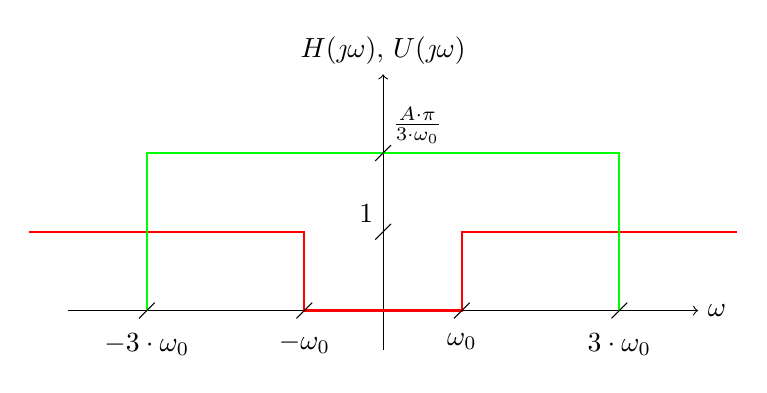
\begin{tikzpicture}
	\draw[->] (-4.0,+0.0) -- (+4.0,+0.0) node[right] {$\omega$};
	\draw[->] (+0.0,-0.5) -- (+0.0,+3.0) node[above] {$H(\jmath \omega)$, $U(\jmath \omega)$};
	\draw[-,red, thick] (-4.5,+1.0) -- (-1.0,1.0) -- (-1.0,+0.0) -- (1.0,+0.0) -- (1.0,+1.0) -- (4.5,1.0);
	\draw[-,green, thick] (-3.0,+0.0) -- (-3.0,2.0) -- (3.0,+2.0) -- (3.0,0.0);
	\draw[-] (-1.0-0.1,-0.1)--(-1.0+0.1,0.1) node[midway, below, outer sep=5pt,align=center] {$-\omega_0$};
	\draw[-] (+1.0-0.1,-0.1)--(+1.0+0.1,0.1) node[midway, below, outer sep=5pt] {$\omega_0$};
	\draw[-] (-3.0-0.1,-0.1)--(-3.0+0.1,0.1) node[midway, below, outer sep=5pt,align=center] {$-3 \cdot \omega_0$};
	\draw[-] (+3.0-0.1,-0.1)--(+3.0+0.1,0.1) node[midway, below, outer sep=5pt] {$3 \cdot \omega_0$};
	
	\draw[-] (-0.1,1.0-0.1)--(+0.1,1.0+0.1) node[midway, above left] {$1$};
	\draw[-] (-0.1,2.0-0.1)--(+0.1,2.0+0.1) node[midway, above right] {$\frac{A \cdot \pi}{3 \cdot \omega_0}$};
	\end{tikzpicture}
\end{figure}

\TT{Teraz dokonujmy operacji mnożenia transformat $U(\jmath \omega)$ przez $H(\jmath \omega)$}{Now, we draw the product of $U(\jmath \omega)$ and $H(\jmath \omega)$:}

\begin{figure}[H]
	\centering
	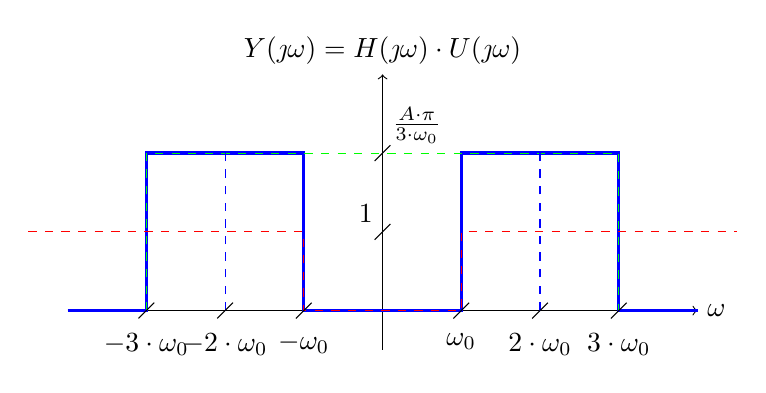
\begin{tikzpicture}
	\draw[->] (-4.0,+0.0) -- (+4.0,+0.0) node[right] {$\omega$};
	\draw[->] (+0.0,-0.5) -- (+0.0,+3.0) node[above] {$Y(\jmath \omega) = H(\jmath \omega) \cdot U(\jmath \omega)$};
	\draw[-,blue, very thick] (-4.0,+0.0) -- (-3.0,+0.0) -- (-3.0,2.0) -- (-1.0,2.0) -- (-1.0,0.0) -- (1.0,0.0) -- (1.0,2.0) --	(3.0,+2.0) -- (3.0,0.0) -- (4.0,0.0);
	
	\draw[-,red, dashed] (-4.5,+1.0) -- (-1.0,1.0) -- (-1.0,+0.0) -- (1.0,+0.0) -- (1.0,+1.0) -- (4.5,1.0);
	\draw[-,green, dashed] (-3.0,+0.0) -- (-3.0,2.0) -- (3.0,+2.0) -- (3.0,0.0);
	
	\draw[-,blue, dashed] (-2.0,+0.0) -- (-2.0,+2.0);
	\draw[-,blue, dashed] (2.0,+0.0) -- (2.0,+2.0);
		
	\draw[-] (-1.0-0.1,-0.1)--(-1.0+0.1,0.1) node[midway, below, outer sep=5pt,align=center] {$-\omega_0$};
	\draw[-] (+1.0-0.1,-0.1)--(+1.0+0.1,0.1) node[midway, below, outer sep=5pt] {$\omega_0$};
	\draw[-] (-3.0-0.1,-0.1)--(-3.0+0.1,0.1) node[midway, below, outer sep=5pt,align=center] {$-3 \cdot \omega_0$};
	\draw[-] (+3.0-0.1,-0.1)--(+3.0+0.1,0.1) node[midway, below, outer sep=5pt] {$3 \cdot \omega_0$};
	\draw[-] (-2.0-0.1,-0.1)--(-2.0+0.1,0.1) node[midway, below, outer sep=5pt,align=center] {$-2 \cdot \omega_0$};
	\draw[-] (+2.0-0.1,-0.1)--(+2.0+0.1,0.1) node[midway, below, outer sep=5pt] {$2 \cdot \omega_0$};
	
	\draw[-] (-0.1,1.0-0.1)--(+0.1,1.0+0.1) node[midway, above left] {$1$};
	\draw[-] (-0.1,2.0-0.1)--(+0.1,2.0+0.1) node[midway, above right] {$\frac{A \cdot \pi}{3 \cdot \omega_0}$};
	\end{tikzpicture}
\end{figure}

\TT{Opiszmy transformatę $Y(\jmath \omega)$ używając sygnałów elementarnych}{The Fourier transform $Y(\jmath \omega)$, using elementary signals, may be described as:}

\begin{equation}
Y(\jmath \omega) = \frac{A \cdot \pi}{3 \cdot \omega_0} \cdot \Pi \left(\frac{\omega - 2 \cdot \omega_0}{2 \cdot \omega_0}\right) +  \frac{A \cdot \pi}{3 \cdot \omega_0} \cdot \Pi \left(\frac{\omega + 2 \cdot \omega_0}{2 \cdot \omega_0}\right)
\end{equation}

\TT{Skoro zanmy transformatę sygnału wyjściowego, to spróbujmy wyznaczyć sygnał wyjściowy w dziedzinie czasu wykorzystując wcześniejsze obliczenia. Transformata $Y(\jmath \omega)$ to suma dwóch przeskalowanych prostokątów, przesuniętych na osi pulsacji. W takim razie można wnioskować, że sygnał w dziedzinie czasiu to będzie suma dwóch zmodulowanych i przeskalowanych funkcji $Sa(t)$.}{Based on earlier calculations, let's try to derive the output $y(t)$ of the system. The $Y(\jmath \omega)$ transform is a sum of two shifted in frequency and scaled rectangular impulses. Based on time-frequency duality theorem, we can expect, that the output $y(t)$ will be a sum of two modulated and scaled $Sa(t)$ signals in the time domain.}

\begin{align*}
\Pi(t) &\xrightarrow{\mathcal F} Sa\left(\frac{\omega}{2}\right)\\
? &\xrightarrow{\mathcal F} \frac{A \cdot \pi}{3 \cdot \omega_0}\cdot \Pi \left(\frac{\omega + 2 \cdot \omega_0}{2 \cdot \omega_0}\right)\\
\end{align*}
 
\begin{align*}
\Pi(t) &\xrightarrow{\mathcal F} Sa\left(\frac{\omega}{2}\right)\\
Sa\left(\frac{t}{2}\right)&\xrightarrow{\mathcal F} 2 \pi \cdot \Pi(-\omega)\\
Sa\left(2 \cdot \omega_0 \cdot \frac{t}{2}\right)&\xrightarrow{\mathcal F} \frac{1}{\left|2 \cdot \omega_0\right|} \cdot 2 \pi \cdot \Pi \left(\frac{\omega}{2 \cdot \omega_0}\right)\\
Sa(\omega_0 \cdot t)&\xrightarrow{\mathcal F} \frac{\pi}{\omega_0}\cdot \Pi \left(\frac{\omega}{2 \cdot \omega_0}\right)\\
e^{(\jmath \cdot 2 \cdot \omega_0 \cdot t)} \cdot Sa(\omega_0 \cdot t)&\xrightarrow{\mathcal F} \frac{\pi}{\omega_0}\cdot \Pi \left(\frac{\omega - 2 \cdot \omega_0}{2 \cdot \omega_0}\right)\\
\frac{A}{3} \cdot e^{(\jmath \cdot 2 \cdot \omega_0 \cdot t)} \cdot Sa(\omega_0 \cdot t)&\xrightarrow{\mathcal F} \frac{A \cdot \pi}{3 \cdot \omega_0}\cdot \Pi \left(\frac{\omega - 2 \cdot \omega_0}{2 \cdot \omega_0}\right)\\
\\
\frac{A}{3} \cdot e^{(\jmath \cdot (-2 \cdot \omega_0) \cdot t)} \cdot Sa(\omega_0 \cdot t)&\xrightarrow{\mathcal F} \frac{A \cdot \pi}{3 \cdot \omega_0}\cdot \Pi \left(\frac{\omega - (-2 \cdot \omega_0)}{2 \cdot \omega_0}\right)\\
\frac{A}{3} \cdot e^{(\jmath \cdot (-2 \cdot \omega_0) \cdot t)} \cdot Sa(\omega_0 \cdot t)&\xrightarrow{\mathcal F} \frac{A \cdot \pi}{3 \cdot \omega_0}\cdot \Pi \left(\frac{\omega + 2 \cdot \omega_0}{2 \cdot \omega_0}\right)\\
\end{align*}

\TT{Podsumowując sygnał wyjściowy $y(t)$:}{To sum up:}
\begin{align*}
y(t) &= \frac{A}{3} \cdot e^{(\jmath \cdot 2 \cdot \omega_0 \cdot t)} \cdot Sa(\omega_0 \cdot t) + \frac{A}{3} \cdot e^{(\jmath \cdot (-2 \cdot \omega_0) \cdot t)} \cdot Sa(\omega_0 \cdot t)=\\
&= \frac{A}{3} \cdot Sa(\omega_0 \cdot t) \cdot \left(e^{(\jmath \cdot 2 \cdot \omega_0 \cdot t)} + e^{(\jmath \cdot (-2 \cdot \omega_0) \cdot t)} \right)=\\
&=\begin{Bmatrix}
\EulerCos
\end{Bmatrix}=\\
&= \frac{2 \cdot A}{3} \cdot Sa(\omega_0 \cdot t) \cdot cos\left(2 \cdot \omega_0 \cdot t)\right)
\end{align*}

\TT{Odpowied\'{z} układu to $y(t)= \frac{2 \cdot A}{3} \cdot Sa(\omega_0 \cdot t) \cdot cos\left(2 \cdot \omega_0 \cdot t\right)$.}{The response of the system is equal to $y(t)= \frac{2 \cdot A}{3} \cdot Sa(\omega_0 \cdot t) \cdot cos\left(2 \cdot \omega_0 \cdot t\right)$.}


\end{task}

